\begin{figure}[H]
    \centering
    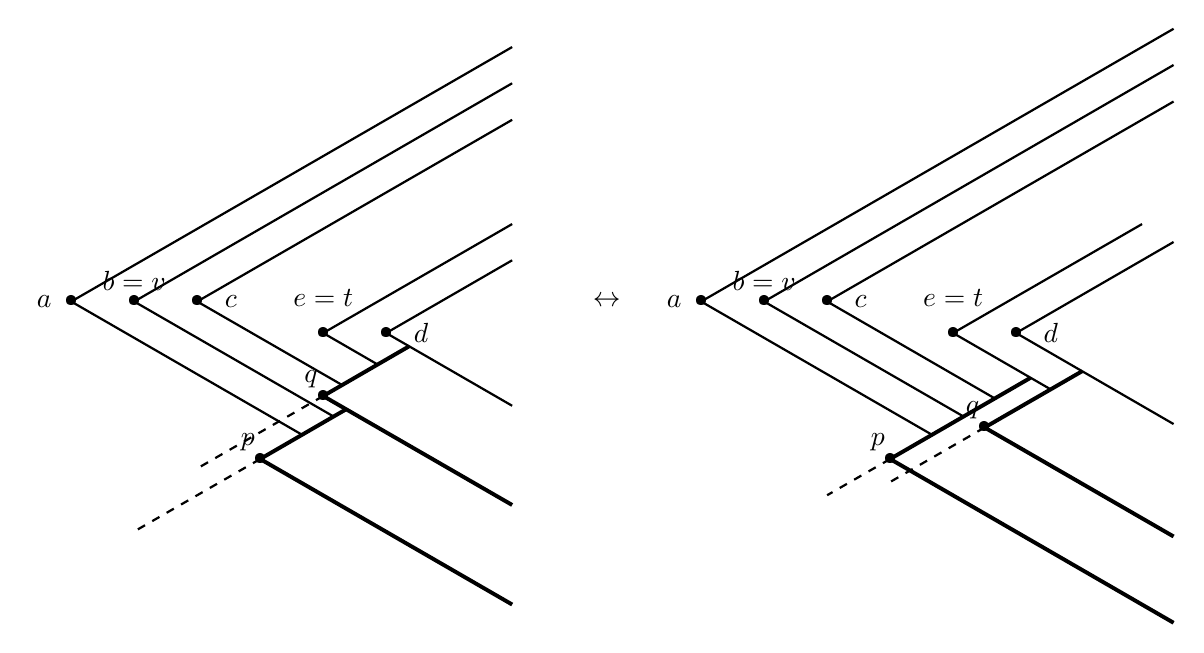
\begin{tikzpicture}[thick, scale=0.4]
        \node[label={[label distance = -3mm]160:$p$}] at
        (6.00, 0.00) {\textbullet};
        \node[label={[label distance = -3mm]160:$q$}] at
        (8.00, 2.00) {\textbullet};
        \node[label={[label distance = -1mm]180:$a$}] at
        (0.00, 5.00) {\textbullet};
        \node[label={[label distance = -2mm]90:$b = v$}] at
        (2.00, 5.00) {\textbullet};
        \node[label={[label distance = 0mm]0:$c$}] at
        (4.00, 5.00) {\textbullet};
        \node[label={[label distance = 0mm]0:$d$}] at
        (10.00, 4.00) {\textbullet};
        \node[label={[label distance = 0mm]90:$e = t$}] at
        (8.00, 4.00) {\textbullet};

        % d cone
        \draw (10.00, 4.00) -- (14.00, 1.69);
        \draw (10.00, 4.00) -- (14.00, 6.31);
        % q cone
        \draw[dashed] (8.00, 2.00) -- (4.00, -0.30);
        \draw[line width = 0.5mm] (8.00, 2.00) -- (14.00, -1.46);
        \draw[line width = 0.5mm] (8.00, 2.00) -- (10.73, 3.58);
        % e cone
        \draw (8.00, 4.00) -- (9.73, 3.00);
        \draw (8.00, 4.00) -- (14.00, 7.46);
        % p cone
        \draw[dashed] (6.00, 0.00) -- (2.00, -2.30);
        \draw[line width = 0.5mm] (6.00, 0.00) -- (14.00, -4.62);
        \draw[line width = 0.5mm] (6.00, 0.00) -- (8.73, 1.58);
        % c cone
        \draw (4.00, 5.00) -- (8.60, 2.35);
        \draw (4.00, 5.00) -- (14.00, 10.77);
        % b cone
        \draw (2.00, 5.00) -- (8.33, 1.35);
        \draw (2.00, 5.00) -- (14.00, 11.93);
        % a cone
        \draw (0.00, 5.00) -- (7.33, 0.77);
        \draw (0.00, 5.00) -- (14.00, 13.08);

        \node at (17, 5) {$ \leftrightarrow$};

        \node[label={[label distance = -3mm]160:$p$}] at
        (26.00, 0.00) {\textbullet};
        \node[label={[label distance = -3mm]160:$q$}] at
        (29.00, 1.00) {\textbullet};
        \node[label={[label distance = -1mm]180:$a$}] at
        (20.00, 5.00) {\textbullet};
        \node[label={[label distance = -2mm]90:$b = v$}] at
        (22.00, 5.00) {\textbullet};
        \node[label={[label distance = 0mm]0:$c$}] at
        (24.00, 5.00) {\textbullet};
        \node[label={[label distance = 0mm]0:$d$}] at
        (30.00, 4.00) {\textbullet};
        \node[label={[label distance = 0mm]90:$e = t$}] at
        (28.00, 4.00) {\textbullet};

        % d cone
        \draw (30.00, 4.00) -- (35.00, 1.11);
        \draw (30.00, 4.00) -- (35.00, 6.89);
        % q cone
        \draw[dashed] (29.00, 1.00) -- (26.00, -0.73);
        \draw[line width = 0.5mm] (29.00, 1.00) -- (35.00, -2.46);
        \draw[line width = 0.5mm] (29.00, 1.00) -- (32.10, 2.79);
        % e cone
        \draw (28.00, 4.00) -- (31.10, 2.21);
        \draw (28.00, 4.00) -- (34.00, 7.46);
        % p cone
        \draw[dashed] (26.00, 0.00) -- (24.00, -1.15);
        \draw[line width = 0.5mm] (26.00, 0.00) -- (35.00, -5.20);
        \draw[line width = 0.5mm] (26.00, 0.00) -- (30.46, 2.58);
        % c cone
        \draw (24.00, 5.00) -- (29.33, 1.92);
        \draw (24.00, 5.00) -- (35.00, 11.35);
        % b cone
        \draw (22.00, 5.00) -- (28.33, 1.35);
        \draw (22.00, 5.00) -- (35.00, 12.51);
        % a cone
        \draw (20.00, 5.00) -- (27.33, 0.77);
        \draw (20.00, 5.00) -- (35.00, 13.66);
    \end{tikzpicture}
    \caption[Exemplo de evento \textsc{down}]{Da esquerda para a direita, o caso em que
    $p$ está em $\Hits_{up}(q)$, ou seja, $q$ está
    entrando em $\Dom(p)$.
    Da direita para a esquerda, o caso em que $q$ está em $\Cands(p)$, saindo de $\Dom(p)$.}
    \label{fig:parcinetico:eventodown}
\end{figure}